\newpage
\section{Images \& tables}
\label{sec:images-tables}

Images and tables can be done following the examples below. Pay attention to the caption position for tables and images. Follow the same format during the label definition for external reference.

\begin{figure}[ht]
    \centering
    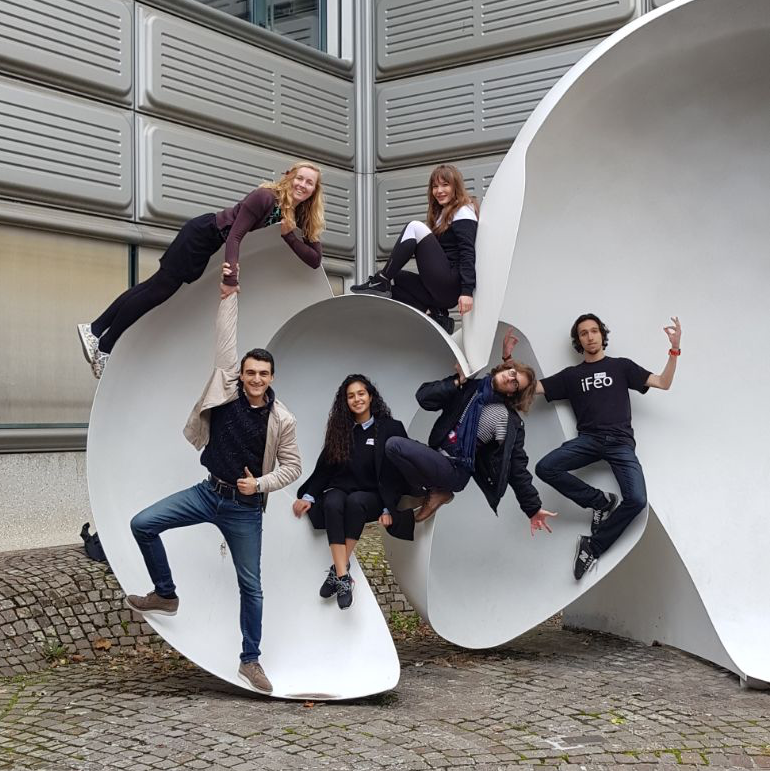
\includegraphics[scale=0.3]{images/CHIC.png}
    \caption{Old but GOLD !}
    \label{fig:CHIC}
\end{figure}

To put two images side by side:
\begin{figure}[H]
    \centering
    \subfloat[Hey, it's us!\label{fig:CHIC1}]{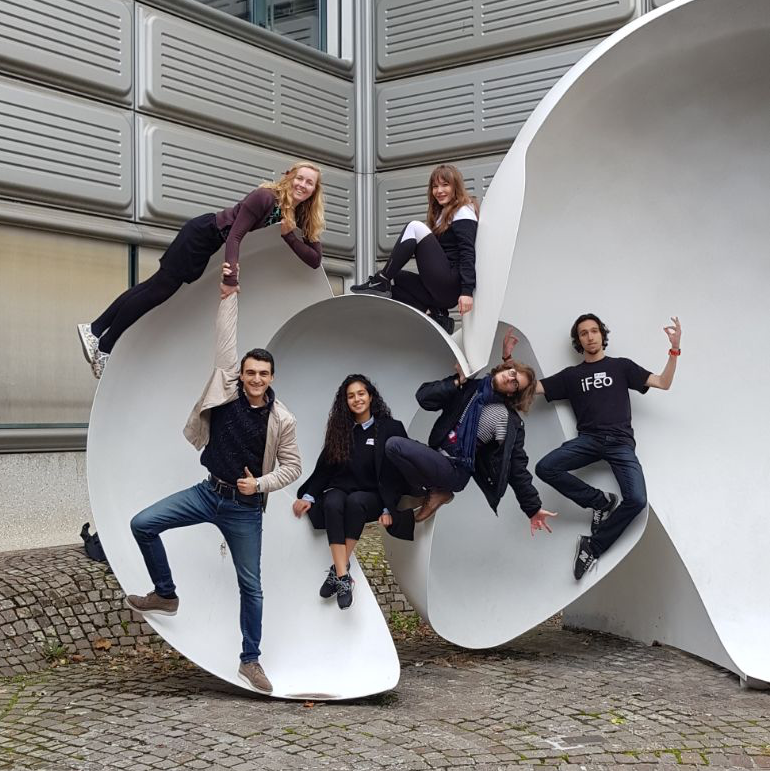
\includegraphics[width=0.45\textwidth]{images/CHIC.png}}\hfill
    \subfloat[Hey, it's us again!\label{fig:CHIC2}] {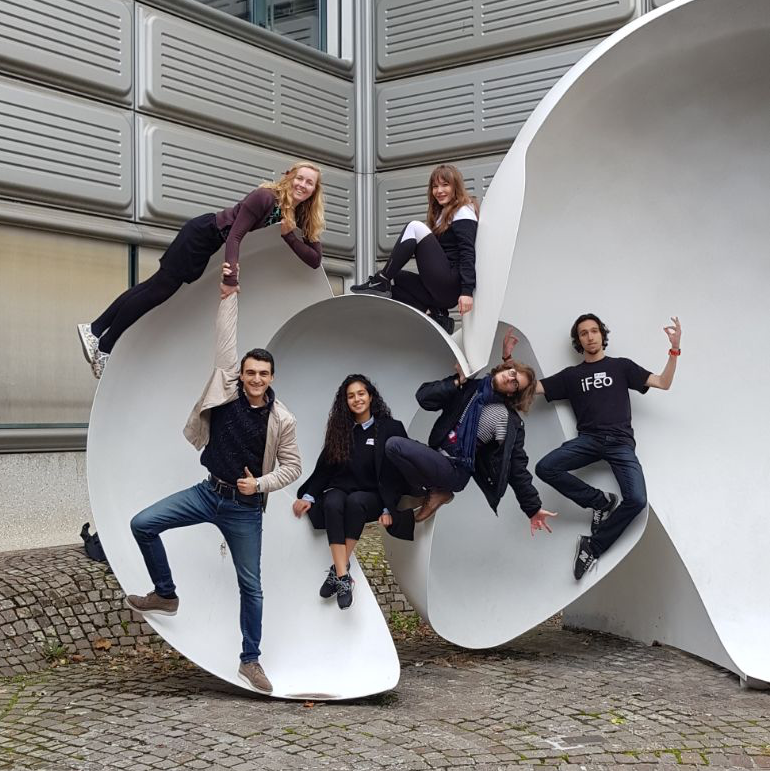
\includegraphics[width=0.5\textwidth]{images/CHIC.png}}\hfill
    \caption{Two for the price of one!} 
    \label{fig:CHIC12}
\end{figure}

\begin{table}[h!]
    \centering
    \caption{Register map of the LCD component}
    \label{tab:register-map}
    \begin{tabular}{ | p{1cm} | p{3.5cm} | p{1cm} | p{1cm} | p{6cm} | }
        \hline
        Offset      & Register name     & R/W   & Size       & Notes \\
        \hline
        \hline
        0   & iRegLength        & W     & 32 bit     &  Stored data length \\
        1   & iRegAddress       & W     & 32 bit     &  Starting address in memory\\
        2   & iRegComParam      & W     & 32 bit     &  Command or Parameter register of LCD \\
        3   & iRegBusy          & R     & 8 bit      &  Display module busy status (cannot receive)\\
        4   & iRegConfigMode    & W     & 8 bit      &  Flag register preparing the Display to receive from the                                                       Slave (not from the FIFO)\\
        5   & iRegState         & R     & 8 bit      &  Current state register of the Display FSM\\
        6   & iRegReset         & W     & 8 bit      &  Reset register to drive the Display resetting\\
        7   & iRegDisplayDone   & R     & 8 bit      &  Register raising a 1 whenever the Display finishes a frame\\
        \hline
    \end{tabular}
\end{table}